\documentclass[12pt]{article} %Basic document type
\usepackage{times} %Font 
\usepackage{amsmath} %For matrices
\usepackage{amssymb}
\usepackage[section]{placeins} %Allows FloatBarrier command
\usepackage[utf8]{inputenc} %Font encoding
\usepackage[margin=1.25in]{geometry} %Adjust margins
\usepackage{graphicx} %Allows picture import
\usepackage{pdfpages} %Including pdf files 
\usepackage{setspace}
\usepackage{fancyhdr}
\usepackage{appendix}
\graphicspath{{images/}} %Allows picture impor
\pagestyle{fancy}
\fancyhf{}
\fancyhead[L]{A Real-Time Object Tracking System}
\fancyhead[R]{ECSE 456}
\fancyfoot[C]{\thepage}
\renewcommand{\headrulewidth}{1pt}
\renewcommand{\footrulewidth}{1.5pt}
\newcommand{\HRule}[1][\medskipamount]{\par
  \vspace*{\dimexpr-\parskip-\baselineskip+#1}
  \noindent\rule{\linewidth}{0.2mm}\par
  \vspace*{\dimexpr-\parskip-.5\baselineskip+#1}}
\begin{document}
\begin{titlepage}
\begin{center}
\textsc{\huge McGill University}\\[1.5cm]
\textsc{\LARGE Department of Electrical \& Computer Engineering}\\[1.5cm]
\textsc{\Large ECSE 456 - Final Report}\\[3cm]
\HRule
{\huge \bfseries A Real-Time Object Tracking System \\[.3cm] }
\HRule 
\vspace{1.5cm}
\noindent
\begin{minipage}{0.4\textwidth}
\begin{flushleft} \large
\emph{\Large Authors:}\\
\vspace{.2cm}
Benjamin \textsc{Brown} \\
\textit{benjamin.brown2@mail.mcgill.ca} \\
260450182 \\
\vspace{.2cm}
Taylor \textsc{Dotsikas} \\
\textit{taylor.dotsikas@mail.mcgill.ca} \\
260457719
\end{flushleft}
\begin{flushleft} \large
\emph{\Large Supervisors:}\\
\vspace{.2cm}
Warren \textsc{Gross, Prof.}\\
\vspace{.2cm}
Arash \textsc{Ardakani} 
\end{flushleft}
\end{minipage}%
\end{center}
\end{titlepage}
\pagebreak
\section*{Abstract}

\section*{Acknowledgments}
The authors would like to thank Professor Warren Gross, for undertaking the responsibility of supervising this project. We also would like to thank Arash Ardakani for all of his advice, help, and time spent meeting with us throughout the semester. Finally, we would also like to thank anyone who contributed to the wealth of online resources about object tracking that we hope to contribute to.
\pagebreak
\tableofcontents
\pagebreak
\section{Abbreviations \& Notation}
\begin{itemize}
\item[] FPGA - Field Programmable Gate Array
\item[] ASIC - Application Specific Integrated Circuit
\item[] CPU - Central Processing Unit
\item[] DFG - Delta Frame Generation
\end{itemize}
\section{Introduction}
\subsection{Motivation}
Ben
\subsection{Applications}
Taylor
\section{Background}
\subsection{Video Processing}
Ben 
\subsection{Optical Flow}
Ben (general) \& Taylor (DFG)
\subsection{Kalman Filter}
Ben
\subsection{Fixed vs. Floating-Point}
Ben
\section{Requirements}
Taylor
\section{Design}
Ben \& Taylor
\subsection{Algorithm}
\subsection{Software}
\begin{figure}[h]
\centering
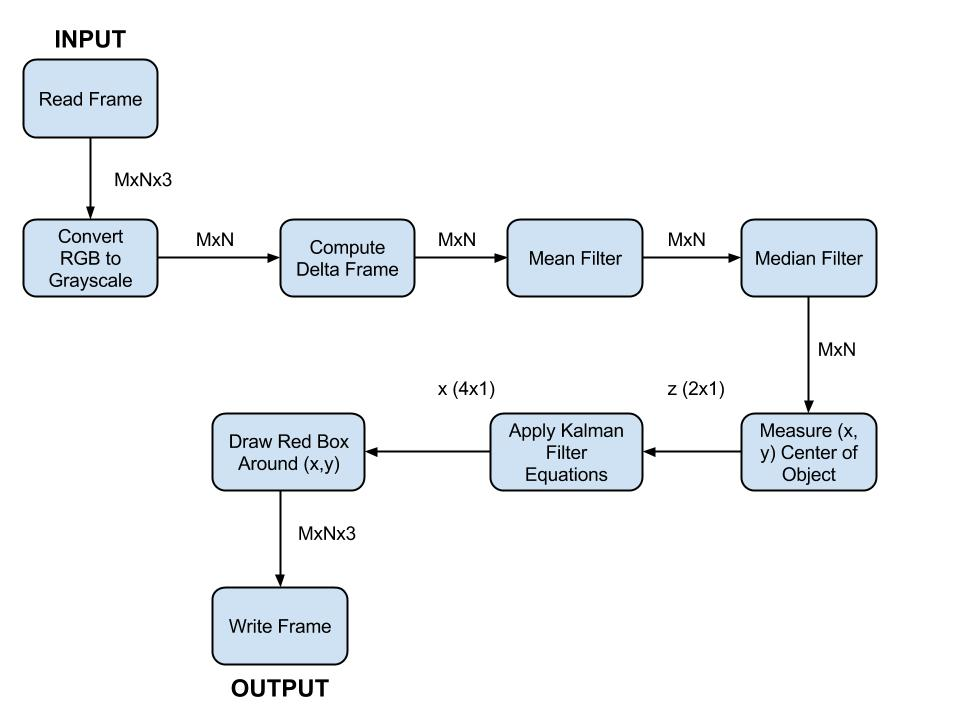
\includegraphics[width=0.75\textwidth]{./images/software_flow.jpg}
\caption{Software Flowchart}
\label{fig:sw_flow}    
\end{figure}
\section{Future Work}
Ben \& Taylor
\section{Impact on Society}
Taylor
\section{Allocation of Work}
Ben \& Taylor
\section{Conclusion}
Ben \& Taylor
\newpage
\begin{thebibliography}{11}
\bibitem{1}
F. Roth, “Using low cost FPGAs for realtime video processing”, M.S. thesis, Faculty of Informatics, Masaryk University, 2011.
\bibitem{2}
A. Saeed et al., “FPGA based Real-time Target Tracking on a Mobile Platform,” in 2010 International Conference on Computational Intelligence and Communication Networks, 2010, pp. 560-564.
\bibitem{3}
”Video and Image Processing Design Using FPGAs.” Altera. 2007. January 2014. 
http://www.altera.com/literature/wp/wp-video0306.pdf  
\bibitem{4}
E. Trucco and A. Verri, “Chapter 8 - Motion,” in Introductory Techniques for 3D Computer, pp. 177- 219.
\bibitem{5}
S.A. El-Azim et al., “An Efficient Object Tracking Technique Using Block-Matching Algorithm”, in Nineteenth National Radio Science Conference, Alexandria, 2002, pp. 427 - 433.
\bibitem{6} 
Caner et al., “An Adaptive Filtering Framework For Image Registration”, IEEE Trans. Acoustics, Speech, and Signal Processing, vol. 2, no. 2, 885-888. March, 2005. 
\bibitem{7}
Yin et al. \textit{Performance Evaluation of Object Tracking Algorithm} [Online]. Available: http://dircweb.kingston.ac.uk/ 
\bibitem{8}
G. Shrikanth, K. Subramanian, “Implementation of FPGA-Based object tracking algorithm,” Electronics and Communication Engineering Sri Venkateswara College of Engineering, 2008.
\bibitem{9}
E. Pizzini, D. Thomas, “FPGA Based Kalman Filter,” Worcester Polytechnic Institute, 2012.
\bibitem{10}
M. Shabany. (2011, December 27). \textit{Floating-point to Fixed-point Conversion} [Online]. Available: http://ee.sharif.edu/~digitalvlsi/Docs/Fixed-Point.pdf
\bibitem{11} 
N. Devillard. (1998, July). \textit{Fast median search: an ANSI C implementation} [Online]. Available: http://ndevilla.free.fr/median/median.pdf
\end{thebibliography}
\newpage
\appendix
\appendixpage
\section{Additional Figures} \label{sec:add}
\end{document}